Interpretability is always a concern for applying deep neural networks
with complicated structures. It is essential for us to make sure that the
CNN taggers we build yield results which at least conform to our physics intuition.
The first cross check performed following the strategy in Ref.~\cite{deOliveira:2015xxd} calculates
the Pearson correlation coefficient of the per pixel intensity with the CNN output score.
As shown in Figure ~\ref{fig:correlation}, the pixel intensity of the core of the image is strongly
 correlated with the output, meaning that the more heavily centered the image is the more likely
the jet is a quark. The intensity of the outer peripheral pixels are anti-correlated with
the CNN output, consistent with the fact that gluon jets tend to have a broader radiation pattern. 

The convolutional filters of CNN can be viewed as capturing features which are distinct to different
class of images. Investigation of these filters will provide useful information of what the CNN regard as
important difference between quarks and gluons. Formally, we examine the difference of applying the
convolutional filters to the average image of quarks($I_q$) and gluons($I_g$), i.e. computing $I_q * w_i - I_g * w_i$,
where $*$ is the convolution operator and $w_i$ denotes the individual filters. The visualizations for the
filters in the first convolutional layer are shown in Figure~\ref{fig:filters}.
Many such difference images are rotational copies of each other as the CNN is able to capture the rotational
invariance. Some of these images are similar to the correlation plot in Figure ~\ref{fig:correlation} suggesting
the radial image difference is one important feature while others are more complex. 

\begin{figure}[htbp]
\begin{center}
\subfloat[][]{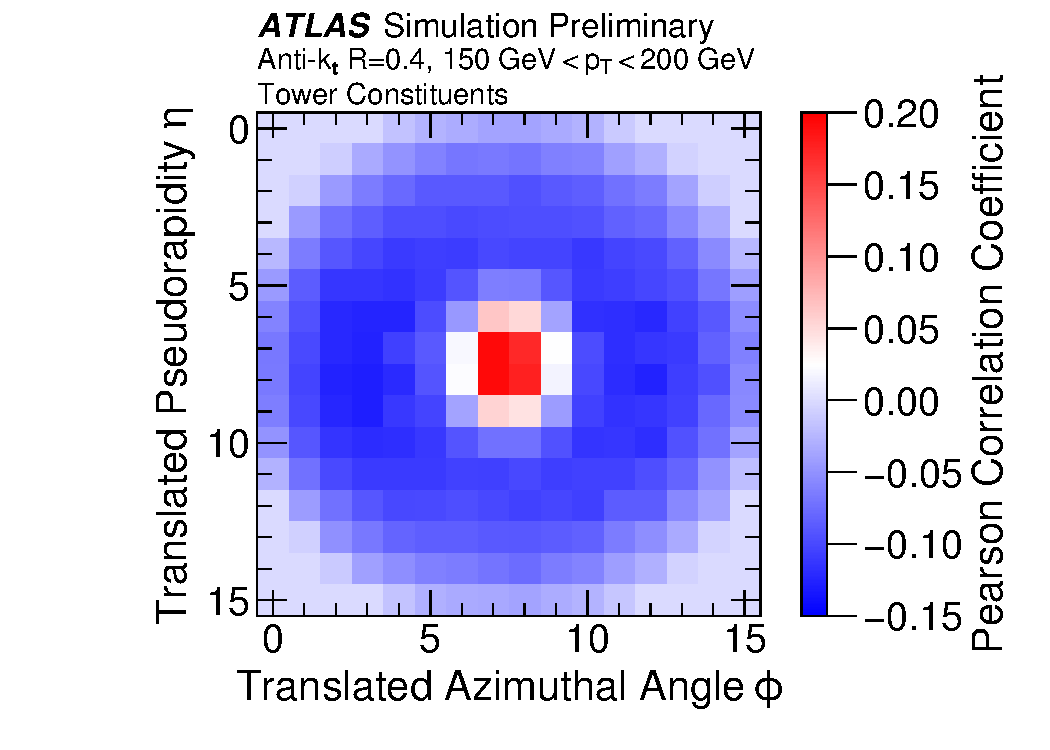
\includegraphics[width=0.7\textwidth]{figures/CNN/corr_tower150200.pdf}}
\caption{
Per-pixel linear correlation with CNN tagger output.
}
\label{fig:correlation}
\end{center}
\end{figure}

\begin{figure}[htbp]
\begin{center}
\subfloat[][]{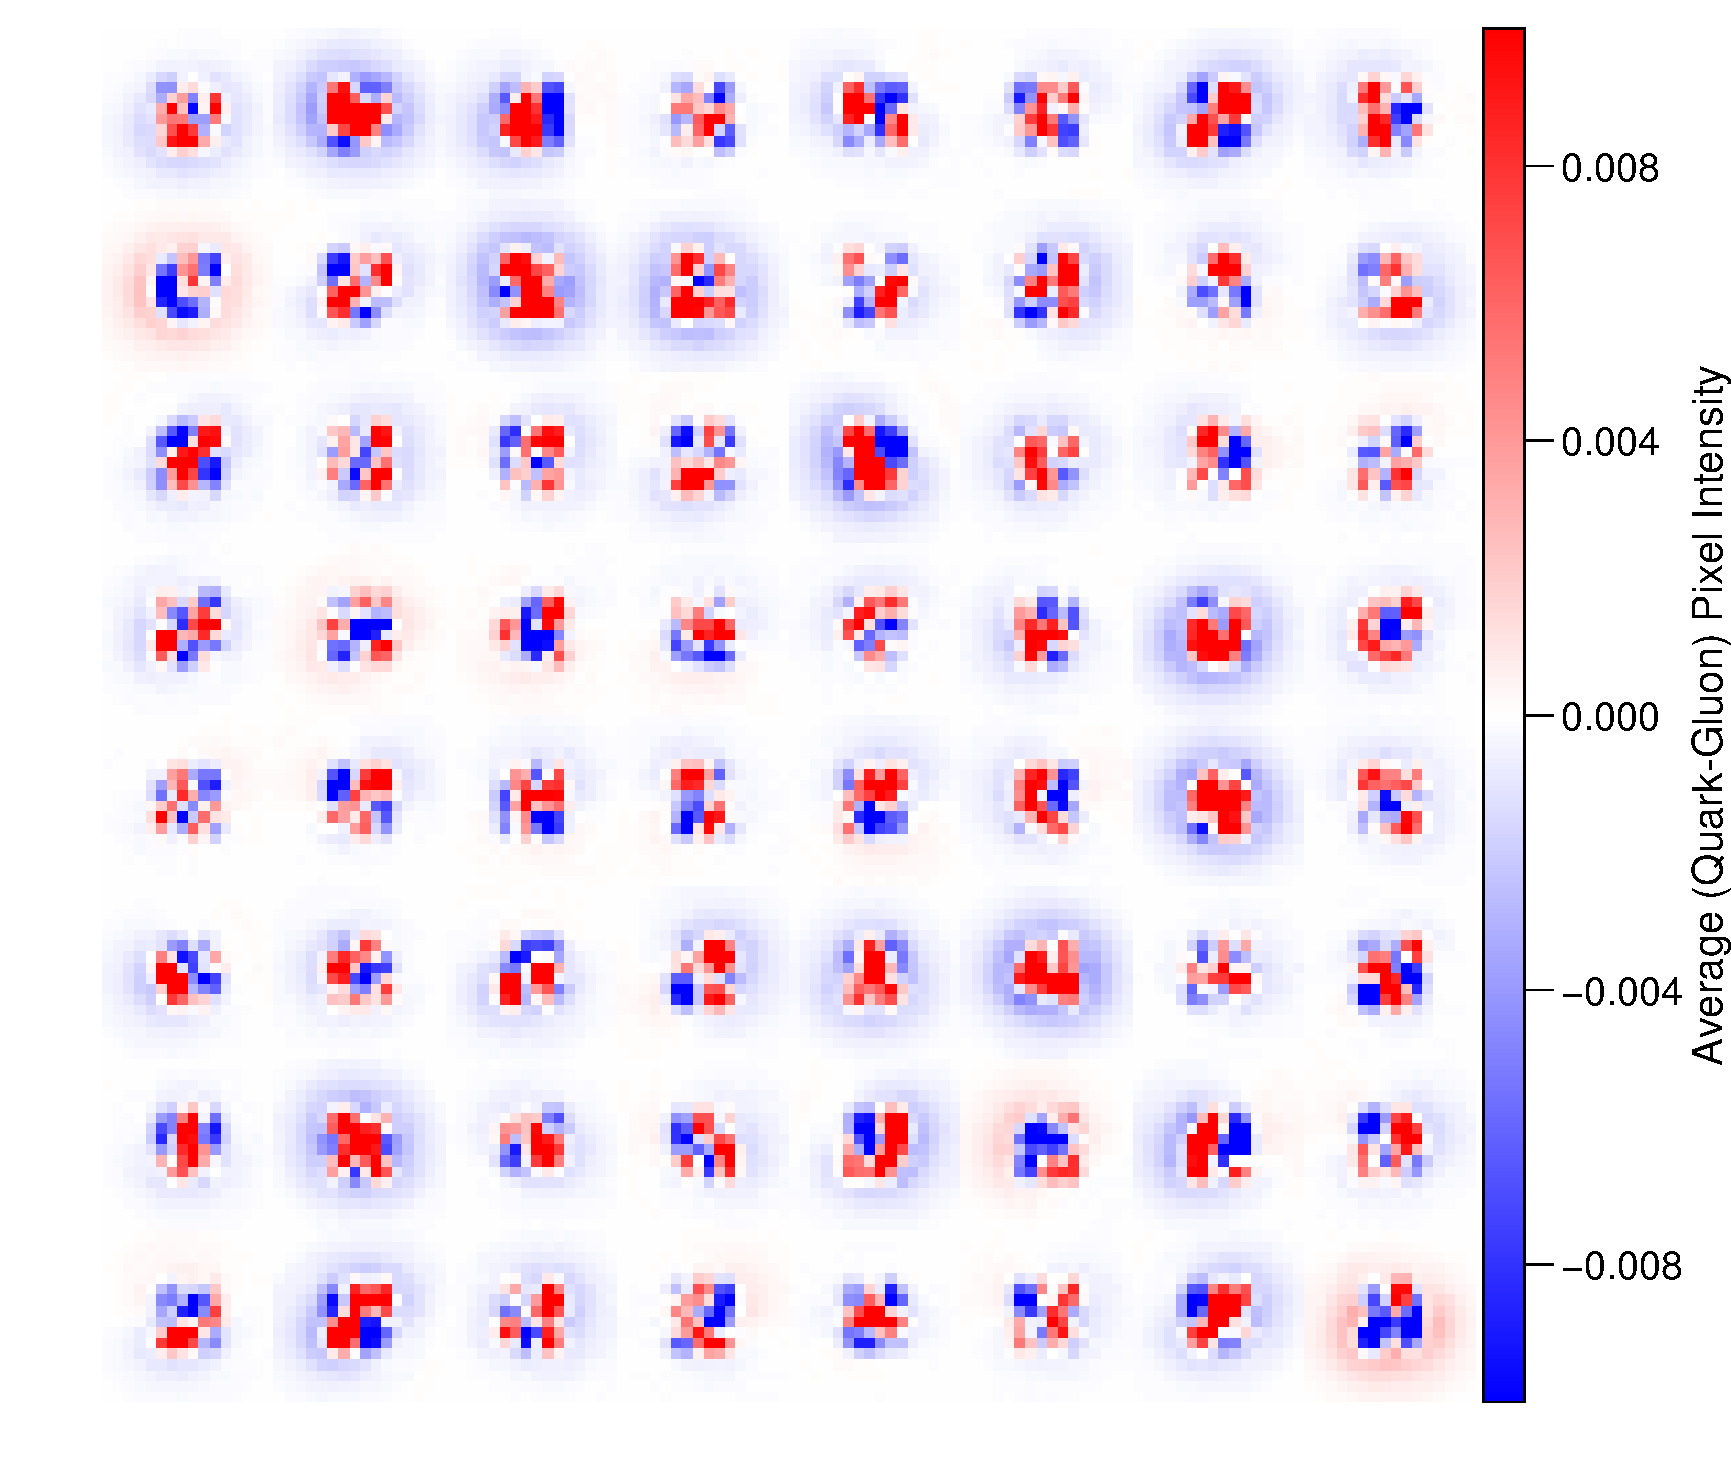
\includegraphics[width=0.9\textwidth]{figures/CNN/convimage_diff.pdf}}
\caption{
Average convolved filter differences for jet images (same color scheme as left plot; red is more quark-like). 
The filters of the first convolutional layer are considered.}
\label{fig:filters}
\end{center}
\end{figure}
